\documentclass{standalone} % Utilise la classe standalone pour compiler uniquement le TikZ
%\include{pakage_tikz}
%\usepackage{tikz}          % Charge le package TikZ
%\usepackage{xcolor}        % Gestion avancée des couleurs
%\usepackage{amsmath}       % Gestion des formules mathématiques
%\usetikzlibrary{arrows.meta} % Pour gérer les flèches avec des formes spécifiées comme "triangle"
%\usetikzlibrary {decorations.pathmorphing}
%%\usepackage{pgfplots}
%%\pgfplotsset{compat=1.18}
%\usepackage[active,tightpage]{preview}
%\PreviewEnvironment{tikzpicture}
%\usetikzlibrary{arrows.meta}
%\usetikzlibrary {arrows.meta,bending,positioning}
%\usetikzlibrary {datavisualization.formats.functions}
%%PREAMBULE pour schÃéma
%\usepackage{pgfplots}
%\usepackage[european resistor, european voltage, european current]{circuitikz}
%\usetikzlibrary{arrows,shapes,positioning}
%\usetikzlibrary{decorations.markings,decorations.pathmorphing,
%decorations.pathreplacing}
%\usetikzlibrary{calc,patterns,shapes.geometric}
%\usepackage{anyfontsize}
%\setlength\PreviewBorder{5pt}


\usepackage{tikz}
\usepackage[european resistor, european voltage, european current]{circuitikz}
\usetikzlibrary{arrows,shapes,positioning}
\usetikzlibrary{decorations.markings,decorations.pathmorphing,
decorations.pathreplacing}
\usetikzlibrary{calc,patterns,shapes.geometric}
\usepackage{anyfontsize}
\usetikzlibrary{patterns,patterns.meta}
%\usepgfplotslibrary{external}
%\tikzexternalize

%% Automatiser cela : une solution plus élégante  nouvelle page, tu peux utiliser la commande \newpage juste avant chaque \begin{tikzpicture}
%\let\oldtikzpicture\tikzpicture
%\let\endoldtikzpicture\endtikzpicture
%\renewenvironment{tikzpicture}{\newpage\oldtikzpicture}{\endoldtikzpicture}
%\usepackage{etoolbox} % dans le préambule, si pas encore utilisé
%\pretocmd{\tikzpicture}{\clearpage}{}{}


% Définition de la fonction pour générer la grille
\newcommand{\drawgrid}[4]{


	\begin{scope}[opacity = 0.2]
	
	
    	% Paramètres : #1=xmin, #2=xmax, #3=ymin, #4=ymax

   	 	% Grille principale en cm
    	\draw[very thin, gray] (#1,#3) grid (#2,#4); % Grille de base (1 cm)
    
    	\draw[very thin, gray] (#1,#3) grid[step=0.1] (#2,#4);

    	\draw[thin, black] (#1,#3) edge[thick,line width=0.8ex,->,>=Stealth ] (#2,#3); 
    
    	\foreach \x in {#1,..., #2} {
        	\draw[shift={(\x, #3)}] (0,-0.1) edge[line width=0.8ex] node[pos = -1 , below] {\x} (0,0.1); % Lignes verticales en mm
    	}

    	\draw[thin, black] (#1,#3)edge[thick,line width=0.8ex,->,>=Stealth ] (#1,#4); 
    
    	\foreach \y in {#3,..., #4} {
        	\draw[shift={(#1, \y)}] (-0.1 , 0 ) edge[line width=0.8ex] node[pos = -1 , left ] {\y} (0.1 , 0); % Lignes verticales en mm
    	}
    
    \end{scope}


}


\newcommand{\Axex}[1][$x$]{ % "x" est la valeur par défaut de #1
    \draw
        (-10, 0) edge[thick, line width=0.8ex, ->, >=Triangle, color=\colorThree] 
        node[shift = {(0,1)} , pos=1.01, below]{ \huge #1 } (10, 0)
        ;
}

\newcommand{\Axetheta}[1][$\theta$]{
	\draw
		(-10, 0 ) edge [thick,line width=0.8ex,->,>=Triangle , color = \colorThree ]node [pos=1.01,right]{\huge #1 } ( 10  , 0 )
	;
}

\newcommand{\Axedensity}[1][$n$]{
	\draw
		(0, -1 ) edge [thick,line width=0.8ex,->,>=Triangle , color = \colorThree ]node [pos=1.01,left  ]{\huge #1 } ( 0  , 6 )
	;
}

\newcommand{\Axedistribution}[1][$\nu$]{
	\draw
		(0, -1 ) edge [thick,line width=0.8ex,->,>=Triangle , color = \colorThree ]node [pos=1.01,left  ]{\huge #1 } ( 0  , 6 )
	;
}

\newcommand{\Axesphase}[2][$x$]{
	\Axex[#1]
	\begin{scope}[rotate = 90]
		\Axetheta[#2]	
	\end{scope}
}

\newcommand{\Axesdensity}[2][$x$]{
	\Axex[#1]
	\Axedensity[#2]
}

\newcommand{\Axesdistribution}[2][\theta]{
	\Axetheta[#1]
	\Axedistribution[#2]
}

\newcommand{\Axetemps}[1][Deformation]{
	\draw 
		(-5 , 0 ) edge [line width=2.8ex, color=\colorOne ]( 0, 0)
		(43 , 0 ) edge [line width=2.8ex, color=\colorOne , ->, >=Triangle] node[pos = 1.0 , right , scale = 2 ] { \fontsize{60pt}{720pt}\selectfont $\tilde{t}$} ( 50 , 0)
		( 0 , 1 ) edge [line width=2.0ex, color=\colorOne ] ( 0 , -1 )  
		( 43 , 1 ) edge [line width=2.0ex, color=\colorOne ] ( 43 , -1 ) 
		(0 , 0) edge[<->, > = stealth, line width=2.8ex, color=\colorOne ]  node [ rectangle , midway, fill = white , scale = 2 ] {\fontsize{600pt}{720pt}\selectfont \bf  #1}(43, 0)  
	;

}

\newcommand{\Palette}[1][\colorOne]{
	\clip[decorate, decoration={random steps, segment length=3pt, amplitude=3pt}]
        	(-1,-1) rectangle (1,1);
	\draw[fill=#1 , color = #1 ] (-2,-2) rectangle (2,2);
}






% Définition des couleurs avec les codes HTML
\definecolor{colorOne}{HTML}{443E46}
%\definecolor{colorTwo}{HTML}{F6DEB8}
\definecolor{colorTwo}{HTML}{FFFFFF}

\definecolor{colorThree}{HTML}{908CA4}
\definecolor{colorFour}{HTML}{57659E}
\definecolor{colorFive}{HTML}{C57284}
\definecolor{colorSix}{HTML}{FF5B69}

% Raccourcis pour les couleurs
\def\colorOne{colorOne}
\def\colorTwo{colorTwo}
\def\colorThree{colorThree}
\def\colorFour{colorFour}
\def\colorFive{colorFive}
\def\colorSix{colorSix}

\definecolor{colorGold}{HTML}{FFD700}
\def\colorGold{colorGold}





\begin{document}

\begin{tikzpicture}
	
% Définition des couleurs avec les codes HTML
\definecolor{colorOne}{HTML}{443E46}
%\definecolor{colorTwo}{HTML}{F6DEB8}
\definecolor{colorTwo}{HTML}{FFFFFF}

\definecolor{colorThree}{HTML}{908CA4}
\definecolor{colorFour}{HTML}{57659E}
\definecolor{colorFive}{HTML}{C57284}
\definecolor{colorSix}{HTML}{FF5B69}

% Raccourcis pour les couleurs
\def\colorOne{colorOne}
\def\colorTwo{colorTwo}
\def\colorThree{colorThree}
\def\colorFour{colorFour}
\def\colorFive{colorFive}
\def\colorSix{colorSix}

\definecolor{colorGold}{HTML}{FFD700}
\def\colorGold{colorGold}



\begin{scope}

	
	%Base L ,S 
	\draw[]
	
		(-1,0) edge [ thick,line width=0.5ex, color = \colorOne ] node [shift={(0cm,-0mm)}, pos = 0.5 , above  ]{{ \color{\colorOne}$5S$}} (1 , 0) 
		
	;
	
	
	% 5S1/2 Fine 	
	\begin{scope}[shift={(1cm,0cm)}]
		\draw
			(0,0) edge [dashed ,line width=0.45ex, color = \colorOne ] (1 , 0)
		;
		
		\begin{scope}[shift={(1cm,0cm)}]
			\draw[shift={(0cm,0cm)}]
				(0,0) edge [ thick,line width=0.5ex, color = \colorOne ] node [shift={(0cm,-1mm)}, pos = 0.75 , above ]{{ \color{\colorOne}$ 5S_{1/2}$}} (2 , 0)
			;
			
			\draw
				(0.25,0.01) edge [decoration={
   							markings,
    						mark connection node=midnode,
    						mark=at position 0.5 with {
      							\node[draw = none ,fill= white ,transform shape , opacity = 1] (midnode) {{\color{\colorFive} \fontsize{8pt}{8pt}\selectfont
					$D_1 : 795~nm$}};
    							}
 						 	},
  							postaction={decorate}, thick, line width=0.5ex, <->, >=Stealth, color=colorFive ] 
   				(0.25,4.29)		
   				(0.75,0.01) edge[decoration={
   							markings,
    						mark connection node=midnode,
    						mark=at position 0.4 with {
      							\node[draw = none ,fill= white ,transform shape , opacity = 1] (midnode) {{\color{\colorFour}\fontsize{8pt}{8pt}\selectfont $D_2 : 780~nm$}};
    							}
 						 	},
  							postaction={decorate}, thick, line width=0.5ex, <->, >=Stealth, color=colorFour ]
   				(0.75,5.74)	
				;
			
			%Hyperfine
			\begin{scope}[shift={(2cm,0cm)}]
				\draw	
					(0,0) edge [dashed ,line width=0.45ex, color = \colorOne ] (1 , 0.75)
					(0,0) edge [dashed ,line width=0.45ex, color = \colorOne ] (1 , -0.75)
				;
				
				\draw[shift={(1cm,0mm)}]
					(0,0.75) edge [ thick,line width=0.5ex, color = \colorOne ] node [shift={(0cm,0mm)}, pos = 1 , right ]{{ \color{\colorOne}$ F = 2 $}} (2 , 0.75)
					(0,-0.75) edge [ thick,line width=0.5ex, color = \colorOne ] node [shift={(0cm,0mm)} , pos = 1 , right ]{{ \color{\colorOne}$ F = 1$}} (2 , -0.75)
				;
				
				
			\end{scope}
		\end{scope}
	\end{scope}
	
	
	% 5P1/2 3/2 Fine 
	\begin{scope}[shift={(1cm,5cm)}]
		
		\draw[shift={(-2cm,0cm)}]
			(0,0) edge [ thick,line width=0.5ex, color = \colorOne ] node [shift={(0cm,-0mm)}, pos = 0.5 , above ]{{ \color{\colorOne}$5P$}} (2 , 0)
		;

		\draw
			(0,0) edge [dashed ,line width=0.45ex, color = \colorOne ] (1 , 0.75)
			(0,0) edge [dashed ,line width=0.45ex, color = \colorOne ] (1 , -0.75)
		;
		
		%5P1/2 
		\begin{scope}[shift={(1cm,-0.75cm)}]		
			\draw
				(0,0) edge [ thick,line width=0.5ex, color = \colorOne ] node [shift={(0cm,-1mm)} , pos = 0.75 , above  ]{{ \color{\colorOne}$ 5P_{1/2}$}} (2 , 0)
			;		
		\end{scope}
		
		%5P3/2 
		\begin{scope}[shift={(1cm,0.75cm)}]		
			\draw
				(0,0) edge [ thick,line width=0.5ex, color = \colorOne ] node [shift={(0cm,-1mm)} , pos = 0.75 , above  ]{{ \color{\colorOne}$ 5P_{3/2}$}} (2 , 0)
			;
			
			%Hyperfine
			\begin{scope}[shift={(2cm,0cm)}]
				\draw
					(0,0) edge [dashed ,line width=0.45ex, color = \colorOne ] (1 , 2.25)
					(0,0) edge [dashed ,line width=0.45ex, color = \colorOne ] (1 , 0.75)
					(0,0) edge [dashed ,line width=0.45ex, color = \colorOne ] (1 , -0.75)
					(0,0) edge [dashed ,line width=0.45ex, color = \colorOne ] (1 , -2.25)
				;
				
				\draw[shift={(1cm,0mm)}]
					(0,2.25) edge [ thick,line width=0.5ex, color = \colorOne ] node [shift={(0cm,0mm)} , pos = 1 , right ]{{ \color{\colorOne}$ F' = 3$}} (2 , 2.25)
					(0,0.75) edge [ thick,line width=0.5ex, color = \colorOne ] node [shift={(0cm,0mm)}, pos = 1 , right ]{{ \color{\colorOne}$ F' = 2 $}} (2 , 0.75)
					(0,-0.75) edge [ thick,line width=0.5ex, color = \colorOne ] node [shift={(0cm,0mm)} , pos = 1 , right ]{{ \color{\colorOne}$ F' = 1$}} (2 , -0.75)
					(0,-2.25) edge [ thick,line width=0.5ex, color = \colorOne ] node [shift={(0cm,0mm)} , pos = 1 , right ]{{ \color{\colorOne}$ F' = 0$}} (2 , -2.25)
					
					(0.55,1.5) edge [dotted ,line width=0.5ex, color = \colorOne ]  (1.45 , 1.5)
					
					(1.25,1.75) edge [dotted ,line width=0.5ex, color = \colorSix ]  (2.15 , 1.75)
					(1.25,2.75) edge [dotted ,line width=0.5ex, color = \colorSix ]  (2.15 , 2.75)
				;
				
				\draw[shift={(1cm,0mm)}]
					(0.25,0.75) edge [decoration={
   							markings,
    						mark connection node=midnode,
    						mark=at position 0.5 with {
      							\node[draw = none ,fill= white ,transform shape , opacity = 1] (midnode) {{\color{\colorFive} \fontsize{4pt}{8pt}\selectfont$267.2~MHz$}};
    							}
 						 	},
  							postaction={decorate}, thick, line width=0.5ex, <->, >=Stealth, color=colorFive ] 
   					(0.25,2.25)		
				;
			\end{scope}		
		\end{scope}
		
	\end{scope}
	
	\draw[shift={(5cm,0mm)}]	
   		(1.75,-0.75) edge[decoration={
   							markings,
    						mark connection node=midnode,
    						mark=at position 0.5 with {
      							\node[draw = none ,fill= white ,transform shape , opacity = 1] (midnode) {{\color{\colorFive}\fontsize{4pt}{8pt}\selectfont $6.874~GHz$}};
    							}
 						 	},
  							postaction={decorate}, thick, line width=0.5ex, <->, >=Stealth, color=colorFive ]
   		(1.75,0.75)
   		(.25,-0.75) edge[decoration={
   							markings,
    						mark connection node=midnode,
    						mark=at position 0.38 with {
      							\node[draw = none ,fill= white ,transform shape , opacity = 1] (midnode) {{\color{\colorSix}\fontsize{8pt}{8pt}\selectfont Repompeur}};
    							}
 						 	},
  							postaction={decorate}, thick, line width=0.5ex, <->, >=Stealth, color=colorSix ]
   		(.25,6.55)	
   		(1.0,0.75) edge[decoration={
   							markings,
    						mark connection node=midnode,
    						mark=at position 0.2 with {
      							\node[draw = none ,fill= white ,transform shape , opacity = 1] (midnode) {{\color{\colorSix}\fontsize{8pt}{8pt}\selectfont Maitre 1}};
    							}
 						 	},
  							postaction={decorate}, thick, line width=0.5ex, <->, >=Stealth, color=colorSix ]
   		(1.0,7.25)	
   		(1.75,0.75) edge[decoration={
   							markings,
    						mark connection node=midnode,
    						mark=at position 0.18 with {
      							\node[draw = none ,fill= white ,transform shape , opacity = 1] (midnode) {{\color{\colorSix}\fontsize{8pt}{8pt}\selectfont Maitre 2 }};
    							}
 						 	},
  							postaction={decorate}, thick, line width=0.5ex, <->, >=Stealth, color=colorSix ]
   		(1.75,7.75)
		;


\end{scope}
							
\end{tikzpicture}

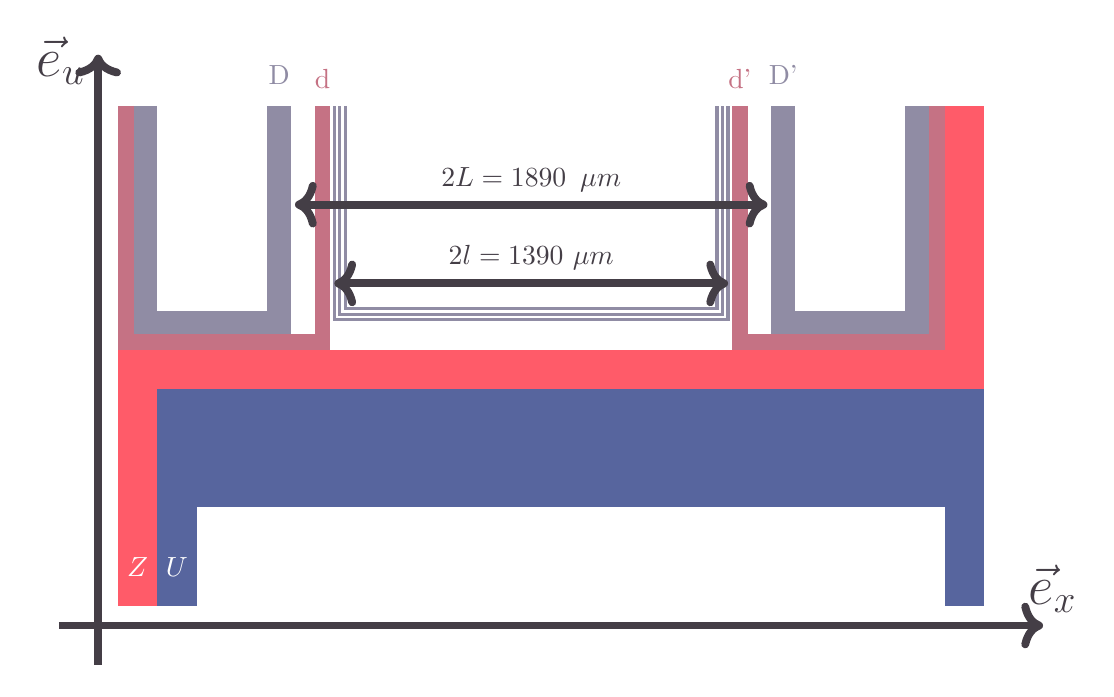
\begin{tikzpicture}
	
% Définition des couleurs avec les codes HTML
\definecolor{colorOne}{HTML}{443E46}
%\definecolor{colorTwo}{HTML}{F6DEB8}
\definecolor{colorTwo}{HTML}{FFFFFF}

\definecolor{colorThree}{HTML}{908CA4}
\definecolor{colorFour}{HTML}{57659E}
\definecolor{colorFive}{HTML}{C57284}
\definecolor{colorSix}{HTML}{FF5B69}

% Raccourcis pour les couleurs
\def\colorOne{colorOne}
\def\colorTwo{colorTwo}
\def\colorThree{colorThree}
\def\colorFour{colorFour}
\def\colorFive{colorFive}
\def\colorSix{colorSix}

\definecolor{colorGold}{HTML}{FFD700}
\def\colorGold{colorGold}


\begin{scope}
	%\drawgrid{-6}{6}{0}{10}	;
	\draw
		(-5,0) edge[thick,line width=0.5cm, color = \colorFour] node [pos = 0 , above]{{\color{\colorTwo} $\bm{U}$}} (-5,2.75)
		(-5,2) edge[thick,line width=1.5cm, color = \colorFour] (5,2)
		(5,2.75) edge[thick,line width=0.5cm, color = \colorFour] (5,0)
	;
	\draw[thick,line width=0.5cm, color = \colorSix]
		(-5.5,0) -- node [pos = 0 , above]{{\color{\colorTwo} $\bm{Z}$}}  (-5.5,3.) -- (5.00,3.0) -- (5.00,6.35)
	;
	\draw[shift={(-5.65cm , 3.35cm)} , thick,line width=0.2cm, color = \colorFive]
		(0,3) -- (0,0)-- (2.5,0)-- node [pos = 1 , above]{d}(2.5,3)
	;
	\draw[shift={(2.15cm , 3.35cm)} , thick,line width=0.2cm, color = \colorFive , opacity = 1]
		(0,3) -- node [pos = 0 , above]{d'} (0,0)-- (2.5,0)-- (2.5,3)
	;
	\draw[shift={(-5.4cm , 3.6cm)} , thick,line width=0.3cm, color = \colorThree , opacity = 1]
		(0,2.75) -- (0,0)-- (1.7,0)-- node [pos = 1 , above]{D} (1.7,2.75)
	;
	\draw[shift={(2.7cm , 3.6cm)} , thick,line width=0.3cm, color = \colorThree , opacity = 1]
		(0,2.75) -- node [pos = 0 , above]{D'} (0,0)-- (1.7,0)-- (1.7,2.75)
	;
	
	\draw[shift={(-3.0cm , 3.6cm)} , thick,line width=0.2cm, color = \colorThree , opacity = 1]
		(0.06,2.75) -- (0.06,0.095)-- (4.94,0.095)-- (4.94,2.75)
	;
	
	\draw[shift={(-3.0cm , 3.6cm)} , thick,line width=0.03cm, color = \colorTwo , opacity = 1]
		(-0.035,2.75) -- (-0.035,0)-- (5.035,0)-- (5.035,2.75)
		(0.035,2.75) -- (0.035,0.07)-- (4.965,0.07)-- (4.965,2.75)
		(0.105,2.75) -- (0.105,0.14)-- (4.895,0.14)-- (4.895,2.75)
	;
	
	\draw[shift={(-3.0cm , 4cm)} , thick,line width=0.1cm, color = \colorOne , opacity = 1 , <->]
		(0.0,0.095) -- node[pos = 0.5, above]{$2l = 1390~\mu m$} (5.0,0.095)
		
	;
	
	\draw[shift={(-3.0cm , 5cm)} , thick,line width=0.1cm, color = \colorOne , opacity = 1 , <->]
		(-0.5,0.095) -- node[pos = 0.5, above]{$2L = 1890 \,\mu m$} (5.5,0.095)
	;
	
	\draw[shift={(-6.0cm , -0.25cm)} , thick,line width=0.1cm, color = \colorOne , opacity = 1 ]
		(-0.5,0)edge[, ->] node[pos = 1.01, above]{\fontsize{20pt}{8pt}\selectfont$\bm{\vec{e}_x}$} (12,0)
		(0,-0.5) edge[, ->] node[pos = 0.99, left]{\fontsize{20pt}{8pt}\selectfont$\bm{\vec{e}_u}$} (0,7.25)
	;
	
\end{scope}
						
\end{tikzpicture}

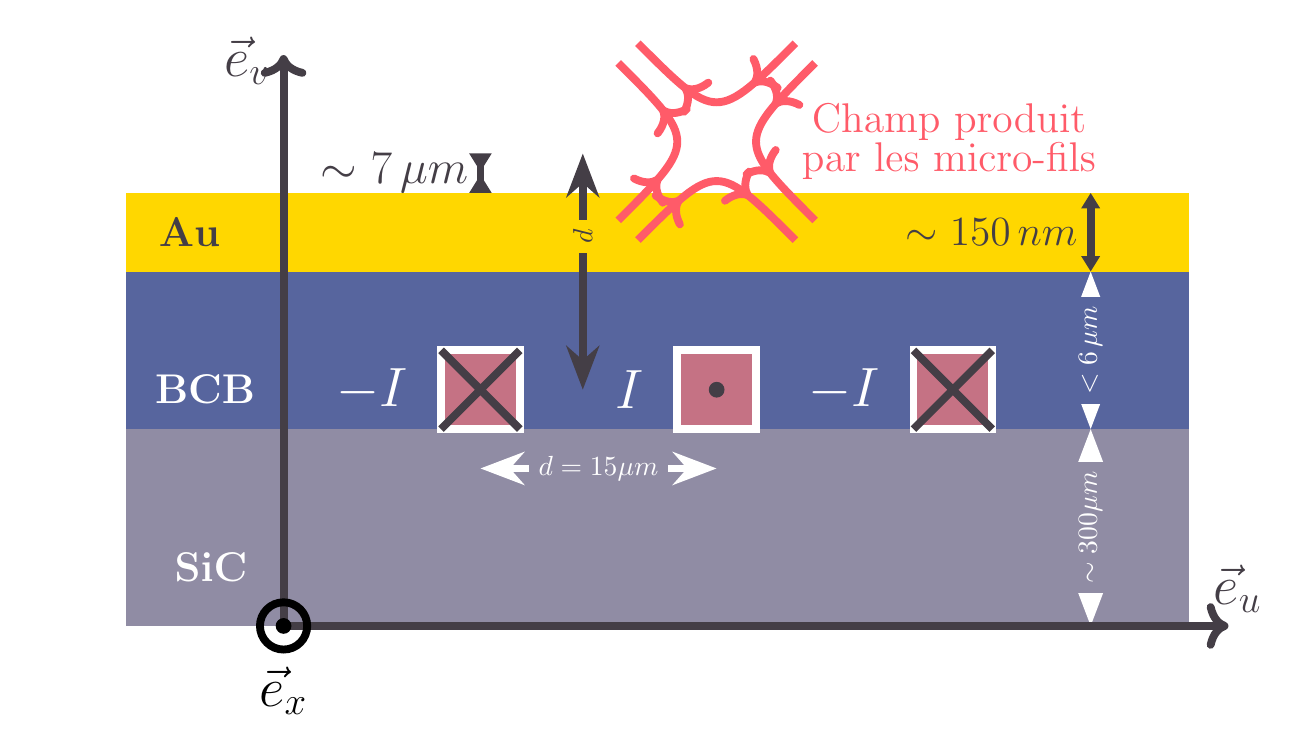
\begin{tikzpicture}
	% Définition des couleurs avec les codes HTML
\definecolor{colorOne}{HTML}{443E46}
%\definecolor{colorTwo}{HTML}{F6DEB8}
\definecolor{colorTwo}{HTML}{FFFFFF}

\definecolor{colorThree}{HTML}{908CA4}
\definecolor{colorFour}{HTML}{57659E}
\definecolor{colorFive}{HTML}{C57284}
\definecolor{colorSix}{HTML}{FF5B69}

% Raccourcis pour les couleurs
\def\colorOne{colorOne}
\def\colorTwo{colorTwo}
\def\colorThree{colorThree}
\def\colorFour{colorFour}
\def\colorFive{colorFive}
\def\colorSix{colorSix}

\definecolor{colorGold}{HTML}{FFD700}
\def\colorGold{colorGold}



\begin{scope}


	\draw[shift={(-2cm , 1.25cm)} , thick,line width=2.5cm, color = \colorThree , opacity = 1 ]
		(0,0) -- node[shift={(-0.75cm , -0.5cm)} , pos = 0.0, right , color = \colorTwo]{{\color{\colorTwo} \fontsize{15pt}{8pt}\selectfont \bf SiC} } (13.5,0)
	;
	\draw[shift={(-2cm , 3.5cm)} , thick,line width=2.cm, color = \colorFour , opacity = 1 ]
		(0,0) -- node[shift={(-0.75cm , -0.5cm)} , pos = 0.0, right , color = \colorTwo]{{\color{\colorTwo} \fontsize{15pt}{8pt}\selectfont \bf BCB} } (13.5,0)
	;
	\draw[shift={(-2cm , 5.cm)} , thick,line width=1.cm, color = \colorGold , opacity = 1 ]
		(0,0) -- node[shift={(-0.2cm , 0.cm)} , pos = 0.0, right , color = \colorTwo]{{\color{\colorOne} \fontsize{15pt}{8pt}\selectfont \bf Au} } (13.5,0)
	;
	
	
	\begin{scope}[shift={(2cm , 2.5cm)}]
		\draw[thick,line width=0.1cm , rounded corners=0cm,  color = \colorTwo , fill = \colorFive ] 
			(0,0) rectangle (1,1)
			;
		% croix
		\draw[ thick,line width=0.1cm , color = \colorOne] 
			(0,0) -- (1,1)
			(0,1) -- (1,0)
		;
		\node[left , shift={(-0.3cm , 0.5cm)} , color = \colorTwo] at (0,0) {{\color{\colorTwo}\fontsize{20pt}{8pt}\selectfont$-I$}};
	\end{scope}
	
	\begin{scope}[shift={(5cm , 2.5cm)}]
		\draw[thick,line width=0.1cm , rounded corners=0cm,  color = \colorTwo , fill = \colorFive ] 
			(0,0) rectangle (1,1)
			;
		% croix
		\fill[ thick,line width=0.1cm , color = \colorOne] 
			(0.5,0.5) circle (0.1cm);
		\node[left , shift={(-0.3cm , 0.5cm)} , color = \colorTwo] at (0,0) {{\color{\colorTwo}\fontsize{20pt}{8pt}\selectfont$I$}};
	\end{scope}
	
	\begin{scope}[shift={(8cm , 2.5cm)}]
		\draw[thick,line width=0.1cm , rounded corners=0cm,  color = \colorTwo , fill = \colorFive ] 
			(0,0) rectangle (1,1)
			;
		% croix
		\draw[ thick,line width=0.1cm , color = \colorOne] 
			(0,0) -- (1,1)
			(0,1) -- (1,0)
		;
		\node[left , shift={(-0.3cm , 0.5cm)} , color = \colorTwo] at (0,0) {{\color{\colorTwo}\fontsize{20pt}{8pt}\selectfont$-I$}};
	\end{scope}
	
	\draw[shift={(2.5cm , 2.cm)}]
		(0,0) edge [decoration={
   							markings,
    						mark connection node=midnode,
    						mark=at position 0.5 with {
      							\node[draw = none ,fill= \colorThree ,transform shape , opacity = 1] (midnode) {{\color{\colorTwo} \fontsize{10pt}{8pt}\selectfont
					$d = 15 \mu m $}};
    							}
 						 	},
  							postaction={decorate},
		thick,line width=0.1cm , <->, color = \colorTwo	, >=Stealth	
		] (3,0)
	;
	
	\draw[shift={(3.8cm , 3.cm)}]
		(0,0) edge [decoration={
   							markings,
    						mark connection node=midnode,
    						mark=at position 0.65 with {
      							\node[draw = none ,fill= \colorGold ,transform shape , opacity = 1] (midnode) {{\color{\colorOne} \fontsize{10pt}{8pt}\selectfont
					$d$}};
    							}
 						 	},
  							postaction={decorate},
		thick,line width=0.1cm , <->, color = \colorOne , >=Stealth	
		] (0,3)
	;
	
	\draw[shift={(10.25cm , 0.cm)}]
		(0,0) edge [decoration={
   							markings,
    						mark connection node=midnode,
    						mark=at position 0.5 with {
      							\node[draw = none ,fill= \colorThree ,transform shape , opacity = 1] (midnode) {{\color{\colorTwo} \fontsize{10pt}{8pt}\selectfont
					$\sim 300 \mu m $}};
    							}
 						 	},
  							postaction={decorate},
		thick,line width=0.1cm , <->, color = \colorTwo	, >=Stealth	
		] (0,2.5)
	;
	
	\draw[shift={(10.25cm , 2.5cm)}]
		(0,0) edge [decoration={
   							markings,
    						mark connection node=midnode,
    						mark=at position 0.5 with {
      							\node[draw = none ,fill= \colorFour ,transform shape , opacity = 1] (midnode) {{\color{\colorTwo} \fontsize{10pt}{8pt}\selectfont
					$< 6 \,\mu m $}};
    							}
 						 	},
  							postaction={decorate},
		thick,line width=0.1cm , <->, color = \colorTwo	, >=Stealth	
		] (0,2)
	;
	
	\draw[shift={(10.25cm , 4.5cm)}, thick,line width=0.1cm , {Triangle[scale=0.5]}-{Triangle[scale=0.5]}, color = \colorOne ]
		(0,0) -- node[pos = 0.5 , left ]{{\color{\colorOne} \fontsize{15pt}{8pt}\selectfont $\sim 150 \, nm $}}  (0,1)
	;
	
	\draw[shift={(2.5cm , 5.5cm)}, thick,line width=0.08cm , >-< ,   {Triangle[scale=0.7, reversed]}-{Triangle[scale=0.7, reversed]}, color = \colorOne ]
		(0,0) -- node[pos = 0.5 , left ]{{\color{\colorOne} \fontsize{17pt}{8pt}\selectfont $\sim 7 \,\mu m $}}  (0,0.5)
	;
	
	\begin{scope}[shift={(4.5cm , 4.9cm)} , decoration={
    		markings,% switch on markings
    		mark=between positions 0.3 and 1 step 1cm with {\arrow[\colorSix,line width=1mm]{>}}}
    	]
  		\draw [postaction={decorate} , color = \colorSix , line width=1mm] (0,0) .. controls (1,1) and (1,1) .. (2,0);
  		\draw [ shift={(2.25cm , 2.25cm)} , rotate = 90, xscale=-1 ,  postaction={decorate} , color = \colorSix , line width=1mm] (0,0) .. controls (1,1) and (1,1) .. (2,0);
  		\draw [shift={(-0.25cm , 0.25cm)} , rotate = -90, xscale=-1 , postaction={decorate} , color = \colorSix , line width=1mm] (0,0) .. controls (1,1) and (1,1) .. (2,0);
  		\draw [shift={(2.cm , 2.5cm)} , rotate = 180, xscale=1 , postaction={decorate} , color = \colorSix , line width=1mm] (0,0) .. controls (1,1) and (1,1) .. (2,0);
  		
  		\node[align=center, font=\fontsize{15}{12}\selectfont, text=\colorSix] at (3.95,1.25) {Champ produit\\par les micro-fils};
	\end{scope}
	

	\draw[shift={(-0.0cm , -0.0cm)} , thick,line width=0.1cm, color = \colorOne , opacity = 1 ]
		(-0.,0)edge[, ->] node[pos = 1.01, above]{\fontsize{20pt}{8pt}\selectfont$\bm{\vec{e}_u}$} (12,0)
		(0,-0.) edge[, ->] node[pos = 0.99, left]{\fontsize{20pt}{8pt}\selectfont$\bm{\vec{e}_v}$} (0,7.25)
	;
	
	\draw[thick ,line width=0.1cm] (0,0) circle (0.3cm);
	\fill (0,0) circle (1mm);
	\node[below , shift={(-0.0cm , -0.4cm)}] at (0,0) {\fontsize{20pt}{8pt}\selectfont$\bm{\vec{e}_x}$};
	
	
	
	%\drawgrid{-3}{12}{-1}{10}
\end{scope}
						
\end{tikzpicture}

\begin{tikzpicture}
	\usetikzlibrary {arrows.meta,petri,positioning}
\usetikzlibrary {backgrounds}
\usetikzlibrary{arrows.meta, petri, positioning, backgrounds, decorations.pathmorphing, fit}

%% Définition des couleurs avec les codes HTML
\definecolor{colorOne}{HTML}{443E46}
%\definecolor{colorTwo}{HTML}{F6DEB8}
\definecolor{colorTwo}{HTML}{FFFFFF}

\definecolor{colorThree}{HTML}{908CA4}
\definecolor{colorFour}{HTML}{57659E}
\definecolor{colorFive}{HTML}{C57284}
\definecolor{colorSix}{HTML}{FF5B69}

% Raccourcis pour les couleurs
\def\colorOne{colorOne}
\def\colorTwo{colorTwo}
\def\colorThree{colorThree}
\def\colorFour{colorFour}
\def\colorFive{colorFive}
\def\colorSix{colorSix}

\definecolor{colorGold}{HTML}{FFD700}


\definecolor{colorPrune}{HTML}{7F004F} % un violet prune profond
\def\colorPrune{colorPrune}

\definecolor{colorGold}{HTML}{FFD700}
\def\colorGold{colorGold}

\tikzset{
  lens/.style={draw, thick, ellipse, minimum width=0.2cm, minimum height=1.2cm},
  mirror/.style={draw, thick, rectangle, minimum width=0.1cm, minimum height=1cm, fill=gray!40},
  laser/.style={draw, thick, rectangle, minimum width=1cm, minimum height=0.4cm, fill=red!20},
}

%\usepackage{tikzoptics}

%\ProvidesPackage{tikzoptics}[2025/07/13 TikZ Optics Elements]
%\RequirePackage{tikz}
\usetikzlibrary{arrows.meta, positioning, calc, decorations.pathmorphing}
\usetikzlibrary{shapes.geometric}

% Couleurs par défaut
\definecolor{laserred}{RGB}{220,20,60}
\definecolor{glassblue}{RGB}{100,100,255}
\definecolor{mirrorgray}{gray}{0.6}

\usepgflibrary {shadings}
% Source laser (boîte)
\tikzset{
  laser source/.style={
    draw, thick, rectangle,
    minimum width=1.2cm, minimum height=0.7cm,
    shading=axis,
    left color=black, right color=black, middle color=colorTwo,
    %top color=black, middle color=white, bottom color=black,
    %outer color=black,inner color=white,
    shading angle=0
  }
}

% Style pour faisceau laser
\tikzset{
  laser beam/.style={
    thick,
    %draw=laserred,
    draw=colorSix, 
    %decoration={snake, amplitude=0.5mm, segment length=2mm},
    %decorate
  }
}
\tikzset{
  sond beam/.style={
    dashed,
    %draw=laserred,
    draw=colorSix, 
    %decoration={snake, amplitude=0.5mm, segment length=2mm},
    %decorate
  }
}


% Fibre optique (cercle)
\tikzset{
  fiber/.style={
    draw = none, thick, circle, minimum size=2.4cm,
    fill= none,
    color = colorSix, 
    path picture={
      \draw[->, thick]
        ([shift={(-0.2,0)}]path picture bounding box.center)
        arc[start angle=-90, end angle=300, radius=0.5cm];
      \draw[->, thick]
        ([shift={(0.2,0)}]path picture bounding box.center)
        arc[start angle=-90, end angle=300, radius=0.5cm];
    }
  }
}


% Lentille convergente (symbole)
\tikzset{
  lens/.style={
    draw = none , thick, fill= none ,
    minimum width=0.2cm, minimum height=1.4cm,
    shape=ellipse,
    path picture={
      \draw[ thick , shading=axis , color = colorFour , left color=colorFour, right color=colorFour, middle color=colorTwo, shading angle=0]
        ([shift={(-0.1,0)}]path picture bounding box.center)
        arc[start angle=180, end angle=170, radius=3.5cm] --++ (0.1, 0 ) 
        arc[start angle=10, end angle=-10, radius=3.5cm] --++ (-0.1 , 0 )
        arc[start angle=-170, end angle=-180, radius=3.5cm] 
       ;
       %\drawgrid{-3}{3}{-1}{3};
    }
  }
}

\usetikzlibrary{patterns.meta}
 %Miroir plan (rectangle vertical incliné)
%\tikzset{
%  mirror/.style={
%    draw = none , thick, fill= none ,
%    minimum width=0.4cm, minimum height=1.4cm,
%    shape=rectangle, rotate=0,
%    path picture={
%      \draw[thick , line width=0.2ex,
%      	color = colorFour , left color=colorFour, right color=white, shading angle=90
%      	]
%        ([shift={(-0.,-0.6)}]path picture bounding box.center)
%        rectangle (0.1,0.6);
%      \fill[
%  		pattern=north west lines,
%  		pattern color=colorFour,
%  		%pattern line width = 0.3pt,     % finesse des traits
%		%pattern scale = 0.5             % plus petit motif
%  		]
%        ([shift={(0.1,-0.6)}]path picture bounding box.center)
%        rectangle ([shift={(0.15,0.6)}]path picture bounding box.center);
%      %\drawgrid{-3}{3}{-1}{3};
%    } 
%  }
%}

%\tikzset{
%  mirror/.style={
%    draw=none, thick, fill=none,
%    minimum width=0.4cm, minimum height=1.4cm,
%    shape=rectangle, rotate=0,
%    path picture={
%      % Bande colorée
%      \draw[thick, line width=0.2ex,
%        color=colorFour, left color=colorFour, right color=white, shading angle=90]
%        ([shift={(-0.,-0.6)}]path picture bounding box.center)
%        rectangle (0.1,0.6);
%
%      % Zone hachurée avec un clip
%      \scope
%        \clip
%          ([shift={(0.1,-0.6)}]path picture bounding box.center)
%          rectangle
%          ([shift={(0.15,0.6)}]path picture bounding box.center);
%
%        % Hachures à 45°
%        \foreach \t in {-1.0,-0.8,...,1.0} {
%          \draw[color=colorFour, line width=0.2pt]
%            ({\t-1},-1) -- ({\t+1},1);
%        }
%      \endscope
%    }
%  }
%}

\tikzset{
  mirror/.style={
    draw=none, line width=1.0pt, fill=none,
    minimum width=0.4cm, minimum height=1.4cm,
    shape=rectangle, rotate=0,
    path picture={
      % Bande colorée
      \draw[thick, line width=0.2ex,
        color=colorFour, left color=colorFour, right color=colorTwo, shading angle=90]
        ([shift={(-0.0,-0.6)}]path picture bounding box.center)
        rectangle (0.1,0.6)
        ([shift={(0.12,-0.615)}]path picture bounding box.center) -- ([shift={(0.12,0.615)}]path picture bounding box.center)
      ;        
      % Hachures à 45° (pas de ligne vide ni de \par)
      \scope
        \clip
          ([shift={(0.1,-0.6)}]path picture bounding box.center)
          rectangle
          ([shift={(0.2,0.6)}]path picture bounding box.center);
        % Hachures à 45°
        \foreach \t in {-1.0,-0.9,...,1.0} {
          \draw[color=colorFour, line width=1.0pt]
            ({\t-1},-1) -- ({\t+1},1);
        }
      \endscope
    }
  }
}


\tikzset{
  sep/.style={
    draw=none, line width=1.0pt, fill=none,
    minimum width=0.4cm, minimum height=1.4cm,
    shape=rectangle, rotate=0,
    path picture={
      % Bande colorée
      \draw[thick, line width=0.2ex,
        rounded corners=0.2ex , color = colorFour , left color=colorFour, right color=colorFour , middle color=colorTwo, shading angle=90]
        ([shift={(-0.0,-0.6)}]path picture bounding box.center)
        rectangle (0.15,0.6)
        %([shift={(0.12,-0.615)}]path picture bounding box.center) -- ([shift={(0.12,0.615)}]path picture bounding box.center)
      ; 
   }
   } 
}



% Lame demi-onde (rectangle avec double flèche)
\tikzset{
  halfwave plate/.style={
    draw , thick, rectangle,
    minimum width=0.2cm, minimum height=1.2cm,
    fill = none,
    line width=0.2ex , rounded corners=0.2ex , color = colorFive , left color=colorFive, right color=colorFive , middle color=colorTwo , shading angle=90,
%    path picture={
%      \draw[ line width=0.2ex , rounded corners=0.5ex , color = colorFive , left color=colorFive, right color=colorFive , middle color=white , shading angle=90]
%        ([xshift=0.1cm, yshift=0.1cm]path picture bounding box.south west)
%          rectangle
%        ([xshift=-0.1cm, yshift=-0.1cm]path picture bounding box.north east);
%    }
  }
}



% TA
\tikzset{
  TA/.style={
    draw = none , thick, rectangle,
    minimum width=1.2cm, minimum height=0.6cm,
    fill = none,
    line width=0.2ex , rounded corners=0.0ex , color = colorOne , left color=colorOne, right color=colorOne , middle color=colorTwo , shading angle=0,
    rotate = 0, 
    path picture={
%       \draw[ line width=0.2ex , rounded corners=0.0ex , color = colorFive , left color=colorFive, right color=colorFive , middle color=colorSix , shading angle=90]
%        ([xshift=0.0cm, yshift=0.01cm]path picture bounding box.west)
%          -- ([xshift=0.0cm, yshift=0.01cm]path picture bounding box.center) --
%        ([xshift=-0.0cm, yshift=0.2cm]path picture bounding box.east) -- ([xshift=-0.0cm, yshift=-0.2cm]path picture bounding box.east) -- ([xshift=0.0cm, yshift=-0.01cm]path picture bounding box.center) --  ([xshift=0.0cm, yshift=-0.01cm]path picture bounding box.west)
%       ;
       \draw[ line width=0.2ex , rounded corners=0.0ex , color = colorFive , left color=colorFive, right color=colorFive , middle color=colorSix , shading angle=90]
        ([xshift=0.0cm, yshift=0.2cm]path picture bounding box.west)
          -- ([xshift=0.0cm, yshift=0.01cm]path picture bounding box.center) --
        ([xshift=-0.0cm, yshift=0.01cm]path picture bounding box.east) -- ([xshift=-0.0cm, yshift=-0.01cm]path picture bounding box.east) -- ([xshift=0.0cm, yshift=-0.01cm]path picture bounding box.center) --  ([xshift=0.0cm, yshift=-0.2cm]path picture bounding box.west)
       ;
    }
  }
}

%      \draw[ line width=0.2ex , rounded corners=0.0ex , color = colorOne , left color=colorOne, right color=colorOne , middle color=colorTwo , shading angle=90]
%        ([xshift=0.1cm, yshift=0.1cm]path picture bounding box.south west)
%          rectangle
%        ([xshift=-0.1cm, yshift=-0.1cm]path picture bounding box.north east)
%       ;

% Lentille cylindrique (ellipse aplatie)
\tikzset{
  cylindrical lens/.style={
    draw = none , thick, fill= none ,
    minimum width=0.2cm, minimum height=1.4cm,
    shape=ellipse,
    path picture={
      \draw[ thick , line width=0.2ex , shading=axis , color = colorFour , left color=colorFour, right color=colorFour, middle color=white, shading angle=0]
        ([shift={(-0.1,0)}]path picture bounding box.center)
        arc[start angle=180, end angle=170, radius=3.5cm] --++ (0.1, 0 ) 
        arc[start angle=10, end angle=-10, radius=3.5cm] --++ (-0.1 , 0 )
        arc[start angle=-170, end angle=-180, radius=3.5cm] 
       ;
       %\drawgrid{-3}{3}{-1}{3};
    }
  }
}

% pignol
\tikzset{
  pignol/.style={
    draw = none , thick, fill= none ,
    minimum width=0.2cm, minimum height=1.4cm,
    shape=ellipse,
    path picture={
      \draw[ thick , line width=0.2ex , color = colorOne]
        ([shift={(0,0)}]path picture bounding box.north) -- ([shift={(0,0.1cm)}]path picture bounding box.center) 
       ;
      \draw[ thick , line width=0.2ex ,  , color = colorOne]
        ([shift={(0,0)}]path picture bounding box.south) -- ([shift={(0,-0.1cm)}]path picture bounding box.center) 
       ;
       %\drawgrid{-3}{3}{-1}{3};
    }
  }
}

% Isolateur optique (boîte avec flèche croisée)
\tikzset{
  optical isolator/.style={
    draw, thick, rectangle, minimum width=1cm, minimum height=0.7cm,
    fill=none ,
    line width=0.2ex , rounded corners=0.0ex , color = colorOne , left color=colorOne, right color=colorOne , middle color=colorTwo , shading angle=90,
    path picture={
      \draw[<-, thick] 
        ([shift={(-0.3,0.2)}]path picture bounding box.center)
        -- ([shift={(0.3,0.2)}]path picture bounding box.center);
        \draw[<-, thick] 
        ([shift={(-0.3,-0.2)}]path picture bounding box.center)
        -- ([shift={(0.3,-0.2)}]path picture bounding box.center);
%      \draw[<-, thick, red] 
%        ([shift={(0.3,-0.3)}]path picture bounding box.center)
%        -- ([shift={(-0.3,-0.3)}]path picture bounding box.center);
    }
  }
}

% Modulateur AOM (boîte avec flèche diagonale)
\tikzset{
  AOM/.style={
    draw, thick, minimum width=0.4cm, minimum height=1cm,
    shape=rectangle, fill=none,
    line width=0.2ex , rounded corners=0.0ex , color = colorOne , left color=colorOne, right color=colorOne , middle color=colorTwo , shading angle=90,
    path picture={
      \fill[pattern=horizontal lines,
  		pattern color=colorOne] 
        ([shift={(0.1,0.1)}]path picture bounding box.south west)
        rectangle ([shift={(-0.1,-0.1)}]path picture bounding box.north east);
    }
  }
}


% Polariseur (rectangle fin + symbole)
\tikzset{
  polarizer/.style={
    draw, thick, minimum width=0.3cm, minimum height=1.4cm,
    fill=gray!30,
    path picture={
      \draw[path picture bounding box]
        ([xshift=-2pt]path picture bounding box.south)
        -- ([xshift=2pt]path picture bounding box.north);
      
    }
  }
}

% Collimateur
\tikzset{
  collimator/.style={
    draw, thick, trapezium, trapezium angle=60,
    minimum height=1cm, fill=blue!10
  }
}


% Miroir dichroïque
\tikzset{
  dichroic/.style={
    draw, thick, fill=yellow!30, rectangle,
    minimum width=0.2cm, minimum height=1.4cm, rotate=45
  }
}

% Détecteur photodiode
\tikzset{
  photodiode/.style={
    draw, thick, regular polygon, regular polygon sides=3, fill=orange!30,
    minimum size=1.2cm, rotate=270
  }
}


% Pinhole (trou)
\tikzset{
  pinhole/.style={
    draw, thick, circle, minimum size=0.3cm, fill=black
  }
}


%DMD
\tikzset{
  DMD/.style={
    draw=none, line width=1.0pt, fill=none,
    minimum width=0.5cm, minimum height=1.5cm,
    shape=rectangle, rotate=0,
    path picture={
      % Bande colorée
      \draw[thick, line width=0.2ex,
        color=colorPrune, left color=colorPrune, right color=white, shading angle=90]
        ([shift={(-0.,-0.7)}]path picture bounding box.center)
        rectangle (0.1,0.7);
      % Hachures à 45° (pas de ligne vide ni de \par)
      \scope
        %\clip
%        \draw[thick]
%          ([shift={(0.1,-0.6)}]path picture bounding box.center)
%          rectangle
%          ([shift={(0.15,0.6)}]path picture bounding box.center);
        % Hachures à 45°
        \def\listetrais{-1.0,-0.9,...,-0.2, 0.1 ,0.2,...,1.0 }
        \def\traity{0.05}
        \def\alpha{12}
        \foreach \t in \listetrais {
		\draw[shift={(1,\t)}, rotate=12, color=colorPrune, line width=0.5pt] 
          ({0.18 - \traity*sin(\alpha)},{\t- \traity*cos(\alpha)}) -- ({0.18 + \traity*sin(\alpha)},{\t+ \traity*cos(\alpha)});
		}
		\def\listetrais{-0.2,-0.1,...,0}
		\foreach \t in \listetrais {
		\draw[shift={(1,\t)}, rotate=12, color=colorPrune, line width=0.5pt] 
          ({0.18 - \traity*sin(-\alpha)},{\t- \traity*cos(-\alpha)}) -- ({0.18 + \traity*sin(-\alpha)},{\t+ \traity*cos(-\alpha)});
		}
      \endscope
    }
  }
}

%lens deme
\tikzset{
  lensd/.style={
    draw = none , thick, fill= none ,
    minimum width=0.2cm, minimum height=1.4cm,
    shape=ellipse,
    path picture={
      \draw[ thick , line width=0.2ex , shading=axis , color = colorFour , left color=colorFour, right color=colorFour, middle color=white, shading angle=0]
        ([shift={(0.0,0.6)}]path picture bounding box.center)
         --++ (0.05, 0 ) 
        arc[start angle=10, end angle=-10, radius=3.5cm] --++ (-0.05 , 0 ) -- cycle
       ;
       %\drawgrid{-3}{3}{-1}{3};
    }
  }
}


%lens deme
\tikzset{
  lensbess/.style={
    draw = none , thick, fill= none ,
    minimum width=1.2cm, minimum height=2.4cm,
    shape=ellipse,
    path picture={
      	\node[lens] (L) {}; 
      	\node[lensd ,  right=-2mm of L]  {};
      	\node[lensd , rotate = 180,  right=-1.5mm of L]  {};
       %\drawgrid{-3}{3}{-1}{3};
    }
  }
}

%lens deme
\tikzset{
  atome/.style={
    draw = red , thick, fill= none ,
    %minimum width=0.1cm, minimum height=0.1cm,
    inner sep=0pt,    % pas de padding interne
    outer sep=0pt,    % pas de marge externe
    %minimum width=0pt, 
    %minimum height=0pt,
    shape=ellipse,
    path picture={
      	\draw[ thick , line width=0.2ex , shading=axis , color = colorFour , left color=colorFour, right color=colorFour, middle color=colorFour, shading angle=0]
      	([shift={(0.0,0)}]path picture bounding box.center) circle (0.3);
       %\drawgrid{-3}{3}{-1}{3};
    }
  }
}


\tikzset{
  CCD/.style={
    draw, thick, rectangle,
    minimum width=1.2cm, minimum height=0.7cm,
    shading=axis,
    left color=colorOne, right color=colorOne, middle color=colorTwo,
    %top color=black, middle color=white, bottom color=black,
    %outer color=black,inner color=white,
    shading angle=0
  }
}


% Définition des couleurs avec les codes HTML
\definecolor{colorOne}{HTML}{443E46}
%\definecolor{colorTwo}{HTML}{F6DEB8}
\definecolor{colorTwo}{HTML}{FFFFFF}

\definecolor{colorThree}{HTML}{908CA4}
\definecolor{colorFour}{HTML}{57659E}
\definecolor{colorFive}{HTML}{C57284}
\definecolor{colorSix}{HTML}{FF5B69}

% Raccourcis pour les couleurs
\def\colorOne{colorOne}
\def\colorTwo{colorTwo}
\def\colorThree{colorThree}
\def\colorFour{colorFour}
\def\colorFive{colorFive}
\def\colorSix{colorSix}

\definecolor{colorGold}{HTML}{FFD700}


\definecolor{colorPrune}{HTML}{7F004F} % un violet prune profond
\def\colorPrune{colorPrune}

\definecolor{colorGold}{HTML}{FFD700}
\def\colorGold{colorGold}

\tikzset{
  lens/.style={draw, thick, ellipse, minimum width=0.2cm, minimum height=1.2cm},
  mirror/.style={draw, thick, rectangle, minimum width=0.1cm, minimum height=1cm, fill=gray!40},
  laser/.style={draw, thick, rectangle, minimum width=1cm, minimum height=0.4cm, fill=red!20},
}

%\usepackage{tikzoptics}

%\ProvidesPackage{tikzoptics}[2025/07/13 TikZ Optics Elements]
%\RequirePackage{tikz}
\usetikzlibrary{arrows.meta, positioning, calc, decorations.pathmorphing}
\usetikzlibrary{shapes.geometric}

% Couleurs par défaut
\definecolor{laserred}{RGB}{220,20,60}
\definecolor{glassblue}{RGB}{100,100,255}
\definecolor{mirrorgray}{gray}{0.6}

\usepgflibrary {shadings}
% Source laser (boîte)
\tikzset{
  laser source/.style={
    draw, thick, rectangle,
    minimum width=1.2cm, minimum height=0.7cm,
    shading=axis,
    left color=black, right color=black, middle color=colorTwo,
    %top color=black, middle color=white, bottom color=black,
    %outer color=black,inner color=white,
    shading angle=0
  }
}

% Style pour faisceau laser
\tikzset{
  laser beam/.style={
    thick,
    %draw=laserred,
    draw=colorSix, 
    %decoration={snake, amplitude=0.5mm, segment length=2mm},
    %decorate
  }
}
\tikzset{
  sond beam/.style={
    dashed,
    %draw=laserred,
    draw=colorSix, 
    %decoration={snake, amplitude=0.5mm, segment length=2mm},
    %decorate
  }
}


% Fibre optique (cercle)
\tikzset{
  fiber/.style={
    draw = none, thick, circle, minimum size=2.4cm,
    fill= none,
    color = colorSix, 
    path picture={
      \draw[->, thick]
        ([shift={(-0.2,0)}]path picture bounding box.center)
        arc[start angle=-90, end angle=300, radius=0.5cm];
      \draw[->, thick]
        ([shift={(0.2,0)}]path picture bounding box.center)
        arc[start angle=-90, end angle=300, radius=0.5cm];
    }
  }
}


% Lentille convergente (symbole)
\tikzset{
  lens/.style={
    draw = none , thick, fill= none ,
    minimum width=0.2cm, minimum height=1.4cm,
    shape=ellipse,
    path picture={
      \draw[ thick , shading=axis , color = colorFour , left color=colorFour, right color=colorFour, middle color=colorTwo, shading angle=0]
        ([shift={(-0.1,0)}]path picture bounding box.center)
        arc[start angle=180, end angle=170, radius=3.5cm] --++ (0.1, 0 ) 
        arc[start angle=10, end angle=-10, radius=3.5cm] --++ (-0.1 , 0 )
        arc[start angle=-170, end angle=-180, radius=3.5cm] 
       ;
       %\drawgrid{-3}{3}{-1}{3};
    }
  }
}

\usetikzlibrary{patterns.meta}
 %Miroir plan (rectangle vertical incliné)
%\tikzset{
%  mirror/.style={
%    draw = none , thick, fill= none ,
%    minimum width=0.4cm, minimum height=1.4cm,
%    shape=rectangle, rotate=0,
%    path picture={
%      \draw[thick , line width=0.2ex,
%      	color = colorFour , left color=colorFour, right color=white, shading angle=90
%      	]
%        ([shift={(-0.,-0.6)}]path picture bounding box.center)
%        rectangle (0.1,0.6);
%      \fill[
%  		pattern=north west lines,
%  		pattern color=colorFour,
%  		%pattern line width = 0.3pt,     % finesse des traits
%		%pattern scale = 0.5             % plus petit motif
%  		]
%        ([shift={(0.1,-0.6)}]path picture bounding box.center)
%        rectangle ([shift={(0.15,0.6)}]path picture bounding box.center);
%      %\drawgrid{-3}{3}{-1}{3};
%    } 
%  }
%}

%\tikzset{
%  mirror/.style={
%    draw=none, thick, fill=none,
%    minimum width=0.4cm, minimum height=1.4cm,
%    shape=rectangle, rotate=0,
%    path picture={
%      % Bande colorée
%      \draw[thick, line width=0.2ex,
%        color=colorFour, left color=colorFour, right color=white, shading angle=90]
%        ([shift={(-0.,-0.6)}]path picture bounding box.center)
%        rectangle (0.1,0.6);
%
%      % Zone hachurée avec un clip
%      \scope
%        \clip
%          ([shift={(0.1,-0.6)}]path picture bounding box.center)
%          rectangle
%          ([shift={(0.15,0.6)}]path picture bounding box.center);
%
%        % Hachures à 45°
%        \foreach \t in {-1.0,-0.8,...,1.0} {
%          \draw[color=colorFour, line width=0.2pt]
%            ({\t-1},-1) -- ({\t+1},1);
%        }
%      \endscope
%    }
%  }
%}

\tikzset{
  mirror/.style={
    draw=none, line width=1.0pt, fill=none,
    minimum width=0.4cm, minimum height=1.4cm,
    shape=rectangle, rotate=0,
    path picture={
      % Bande colorée
      \draw[thick, line width=0.2ex,
        color=colorFour, left color=colorFour, right color=colorTwo, shading angle=90]
        ([shift={(-0.0,-0.6)}]path picture bounding box.center)
        rectangle (0.1,0.6)
        ([shift={(0.12,-0.615)}]path picture bounding box.center) -- ([shift={(0.12,0.615)}]path picture bounding box.center)
      ;        
      % Hachures à 45° (pas de ligne vide ni de \par)
      \scope
        \clip
          ([shift={(0.1,-0.6)}]path picture bounding box.center)
          rectangle
          ([shift={(0.2,0.6)}]path picture bounding box.center);
        % Hachures à 45°
        \foreach \t in {-1.0,-0.9,...,1.0} {
          \draw[color=colorFour, line width=1.0pt]
            ({\t-1},-1) -- ({\t+1},1);
        }
      \endscope
    }
  }
}


\tikzset{
  sep/.style={
    draw=none, line width=1.0pt, fill=none,
    minimum width=0.4cm, minimum height=1.4cm,
    shape=rectangle, rotate=0,
    path picture={
      % Bande colorée
      \draw[thick, line width=0.2ex,
        rounded corners=0.2ex , color = colorFour , left color=colorFour, right color=colorFour , middle color=colorTwo, shading angle=90]
        ([shift={(-0.0,-0.6)}]path picture bounding box.center)
        rectangle (0.15,0.6)
        %([shift={(0.12,-0.615)}]path picture bounding box.center) -- ([shift={(0.12,0.615)}]path picture bounding box.center)
      ; 
   }
   } 
}



% Lame demi-onde (rectangle avec double flèche)
\tikzset{
  halfwave plate/.style={
    draw , thick, rectangle,
    minimum width=0.2cm, minimum height=1.2cm,
    fill = none,
    line width=0.2ex , rounded corners=0.2ex , color = colorFive , left color=colorFive, right color=colorFive , middle color=colorTwo , shading angle=90,
%    path picture={
%      \draw[ line width=0.2ex , rounded corners=0.5ex , color = colorFive , left color=colorFive, right color=colorFive , middle color=white , shading angle=90]
%        ([xshift=0.1cm, yshift=0.1cm]path picture bounding box.south west)
%          rectangle
%        ([xshift=-0.1cm, yshift=-0.1cm]path picture bounding box.north east);
%    }
  }
}



% TA
\tikzset{
  TA/.style={
    draw = none , thick, rectangle,
    minimum width=1.2cm, minimum height=0.6cm,
    fill = none,
    line width=0.2ex , rounded corners=0.0ex , color = colorOne , left color=colorOne, right color=colorOne , middle color=colorTwo , shading angle=0,
    rotate = 0, 
    path picture={
%       \draw[ line width=0.2ex , rounded corners=0.0ex , color = colorFive , left color=colorFive, right color=colorFive , middle color=colorSix , shading angle=90]
%        ([xshift=0.0cm, yshift=0.01cm]path picture bounding box.west)
%          -- ([xshift=0.0cm, yshift=0.01cm]path picture bounding box.center) --
%        ([xshift=-0.0cm, yshift=0.2cm]path picture bounding box.east) -- ([xshift=-0.0cm, yshift=-0.2cm]path picture bounding box.east) -- ([xshift=0.0cm, yshift=-0.01cm]path picture bounding box.center) --  ([xshift=0.0cm, yshift=-0.01cm]path picture bounding box.west)
%       ;
       \draw[ line width=0.2ex , rounded corners=0.0ex , color = colorFive , left color=colorFive, right color=colorFive , middle color=colorSix , shading angle=90]
        ([xshift=0.0cm, yshift=0.2cm]path picture bounding box.west)
          -- ([xshift=0.0cm, yshift=0.01cm]path picture bounding box.center) --
        ([xshift=-0.0cm, yshift=0.01cm]path picture bounding box.east) -- ([xshift=-0.0cm, yshift=-0.01cm]path picture bounding box.east) -- ([xshift=0.0cm, yshift=-0.01cm]path picture bounding box.center) --  ([xshift=0.0cm, yshift=-0.2cm]path picture bounding box.west)
       ;
    }
  }
}

%      \draw[ line width=0.2ex , rounded corners=0.0ex , color = colorOne , left color=colorOne, right color=colorOne , middle color=colorTwo , shading angle=90]
%        ([xshift=0.1cm, yshift=0.1cm]path picture bounding box.south west)
%          rectangle
%        ([xshift=-0.1cm, yshift=-0.1cm]path picture bounding box.north east)
%       ;

% Lentille cylindrique (ellipse aplatie)
\tikzset{
  cylindrical lens/.style={
    draw = none , thick, fill= none ,
    minimum width=0.2cm, minimum height=1.4cm,
    shape=ellipse,
    path picture={
      \draw[ thick , line width=0.2ex , shading=axis , color = colorFour , left color=colorFour, right color=colorFour, middle color=white, shading angle=0]
        ([shift={(-0.1,0)}]path picture bounding box.center)
        arc[start angle=180, end angle=170, radius=3.5cm] --++ (0.1, 0 ) 
        arc[start angle=10, end angle=-10, radius=3.5cm] --++ (-0.1 , 0 )
        arc[start angle=-170, end angle=-180, radius=3.5cm] 
       ;
       %\drawgrid{-3}{3}{-1}{3};
    }
  }
}

% pignol
\tikzset{
  pignol/.style={
    draw = none , thick, fill= none ,
    minimum width=0.2cm, minimum height=1.4cm,
    shape=ellipse,
    path picture={
      \draw[ thick , line width=0.2ex , color = colorOne]
        ([shift={(0,0)}]path picture bounding box.north) -- ([shift={(0,0.1cm)}]path picture bounding box.center) 
       ;
      \draw[ thick , line width=0.2ex ,  , color = colorOne]
        ([shift={(0,0)}]path picture bounding box.south) -- ([shift={(0,-0.1cm)}]path picture bounding box.center) 
       ;
       %\drawgrid{-3}{3}{-1}{3};
    }
  }
}

% Isolateur optique (boîte avec flèche croisée)
\tikzset{
  optical isolator/.style={
    draw, thick, rectangle, minimum width=1cm, minimum height=0.7cm,
    fill=none ,
    line width=0.2ex , rounded corners=0.0ex , color = colorOne , left color=colorOne, right color=colorOne , middle color=colorTwo , shading angle=90,
    path picture={
      \draw[<-, thick] 
        ([shift={(-0.3,0.2)}]path picture bounding box.center)
        -- ([shift={(0.3,0.2)}]path picture bounding box.center);
        \draw[<-, thick] 
        ([shift={(-0.3,-0.2)}]path picture bounding box.center)
        -- ([shift={(0.3,-0.2)}]path picture bounding box.center);
%      \draw[<-, thick, red] 
%        ([shift={(0.3,-0.3)}]path picture bounding box.center)
%        -- ([shift={(-0.3,-0.3)}]path picture bounding box.center);
    }
  }
}

% Modulateur AOM (boîte avec flèche diagonale)
\tikzset{
  AOM/.style={
    draw, thick, minimum width=0.4cm, minimum height=1cm,
    shape=rectangle, fill=none,
    line width=0.2ex , rounded corners=0.0ex , color = colorOne , left color=colorOne, right color=colorOne , middle color=colorTwo , shading angle=90,
    path picture={
      \fill[pattern=horizontal lines,
  		pattern color=colorOne] 
        ([shift={(0.1,0.1)}]path picture bounding box.south west)
        rectangle ([shift={(-0.1,-0.1)}]path picture bounding box.north east);
    }
  }
}


% Polariseur (rectangle fin + symbole)
\tikzset{
  polarizer/.style={
    draw, thick, minimum width=0.3cm, minimum height=1.4cm,
    fill=gray!30,
    path picture={
      \draw[path picture bounding box]
        ([xshift=-2pt]path picture bounding box.south)
        -- ([xshift=2pt]path picture bounding box.north);
      
    }
  }
}

% Collimateur
\tikzset{
  collimator/.style={
    draw, thick, trapezium, trapezium angle=60,
    minimum height=1cm, fill=blue!10
  }
}


% Miroir dichroïque
\tikzset{
  dichroic/.style={
    draw, thick, fill=yellow!30, rectangle,
    minimum width=0.2cm, minimum height=1.4cm, rotate=45
  }
}

% Détecteur photodiode
\tikzset{
  photodiode/.style={
    draw, thick, regular polygon, regular polygon sides=3, fill=orange!30,
    minimum size=1.2cm, rotate=270
  }
}


% Pinhole (trou)
\tikzset{
  pinhole/.style={
    draw, thick, circle, minimum size=0.3cm, fill=black
  }
}


%DMD
\tikzset{
  DMD/.style={
    draw=none, line width=1.0pt, fill=none,
    minimum width=0.5cm, minimum height=1.5cm,
    shape=rectangle, rotate=0,
    path picture={
      % Bande colorée
      \draw[thick, line width=0.2ex,
        color=colorPrune, left color=colorPrune, right color=white, shading angle=90]
        ([shift={(-0.,-0.7)}]path picture bounding box.center)
        rectangle (0.1,0.7);
      % Hachures à 45° (pas de ligne vide ni de \par)
      \scope
        %\clip
%        \draw[thick]
%          ([shift={(0.1,-0.6)}]path picture bounding box.center)
%          rectangle
%          ([shift={(0.15,0.6)}]path picture bounding box.center);
        % Hachures à 45°
        \def\listetrais{-1.0,-0.9,...,-0.2, 0.1 ,0.2,...,1.0 }
        \def\traity{0.05}
        \def\alpha{12}
        \foreach \t in \listetrais {
		\draw[shift={(1,\t)}, rotate=12, color=colorPrune, line width=0.5pt] 
          ({0.18 - \traity*sin(\alpha)},{\t- \traity*cos(\alpha)}) -- ({0.18 + \traity*sin(\alpha)},{\t+ \traity*cos(\alpha)});
		}
		\def\listetrais{-0.2,-0.1,...,0}
		\foreach \t in \listetrais {
		\draw[shift={(1,\t)}, rotate=12, color=colorPrune, line width=0.5pt] 
          ({0.18 - \traity*sin(-\alpha)},{\t- \traity*cos(-\alpha)}) -- ({0.18 + \traity*sin(-\alpha)},{\t+ \traity*cos(-\alpha)});
		}
      \endscope
    }
  }
}

%lens deme
\tikzset{
  lensd/.style={
    draw = none , thick, fill= none ,
    minimum width=0.2cm, minimum height=1.4cm,
    shape=ellipse,
    path picture={
      \draw[ thick , line width=0.2ex , shading=axis , color = colorFour , left color=colorFour, right color=colorFour, middle color=white, shading angle=0]
        ([shift={(0.0,0.6)}]path picture bounding box.center)
         --++ (0.05, 0 ) 
        arc[start angle=10, end angle=-10, radius=3.5cm] --++ (-0.05 , 0 ) -- cycle
       ;
       %\drawgrid{-3}{3}{-1}{3};
    }
  }
}


%lens deme
\tikzset{
  lensbess/.style={
    draw = none , thick, fill= none ,
    minimum width=1.2cm, minimum height=2.4cm,
    shape=ellipse,
    path picture={
      	\node[lens] (L) {}; 
      	\node[lensd ,  right=-2mm of L]  {};
      	\node[lensd , rotate = 180,  right=-1.5mm of L]  {};
       %\drawgrid{-3}{3}{-1}{3};
    }
  }
}

%lens deme
\tikzset{
  atome/.style={
    draw = red , thick, fill= none ,
    %minimum width=0.1cm, minimum height=0.1cm,
    inner sep=0pt,    % pas de padding interne
    outer sep=0pt,    % pas de marge externe
    %minimum width=0pt, 
    %minimum height=0pt,
    shape=ellipse,
    path picture={
      	\draw[ thick , line width=0.2ex , shading=axis , color = colorFour , left color=colorFour, right color=colorFour, middle color=colorFour, shading angle=0]
      	([shift={(0.0,0)}]path picture bounding box.center) circle (0.3);
       %\drawgrid{-3}{3}{-1}{3};
    }
  }
}


\tikzset{
  CCD/.style={
    draw, thick, rectangle,
    minimum width=1.2cm, minimum height=0.7cm,
    shading=axis,
    left color=colorOne, right color=colorOne, middle color=colorTwo,
    %top color=black, middle color=white, bottom color=black,
    %outer color=black,inner color=white,
    shading angle=0
  }
}




\begin{scope}[node distance=1.8cm and 1.2cm]

	
	\node[DMD] at (0,0) (DMD) {};
	\node[left=-1mm of DMD, rotate=90, anchor=center , color = \colorPrune] (DMDlabel) { \color{\colorPrune} \small DMD};
				
	\node[lens ,  right=20mm of DMD] (lensDMD) {};
	
	
	
	
	\node[,  right=25mm of lensDMD ] (mirrord1) {
  		\begin{tikzpicture}
  			\draw[mirror , rotate = 45];
  		\end{tikzpicture}
  	};
  	
  	
  	\node[fiber ,  above=0mm of mirrord1 , shift = {(-0.1,0)} , rotate = 16 ,  xscale = -1 ] (fibre) {};
  	
  	\node[right=2mm of mirrord1, shift = {(0,1.62)}] (In) {};
  
  	\node[scale=0.3, rotate=16 , shift = {(0,-0.5)} ]  at ($(In)!0.15!(DMD)$) {\color{\colorSix} fibre};
  	\node[lens, scale=0.3, rotate=16] (collimateur) at ($(In)!0.25!(DMD)$) {};
  	\node[scale=0.3, rotate=16 , shift = {(0,-1)} ]  at ($(In)!0.25!(DMD)$) {\color{\colorFour} collimateur};
  	\node[lens, scale=0.5, rotate=16] (lens1) at ($(In)!0.35!(DMD)$) {};
  	\node[halfwave plate, scale=0.4, rotate=16] () at ($(In)!0.4!(DMD)$) {};
  	\node[ scale=0.4, rotate=16 , shift = {(0,-1)} ] () at ($(In)!0.4!(DMD)$) {\color{\colorSix}$\lambda/2$};
  	\node[lens, scale=0.5, rotate=16] () at ($(In)!0.45!(DMD)$) {};
  	
  	
  	\node[,  below=25mm of mirrord1] (Sep) {
  		\begin{tikzpicture}
  			\draw[sep , rotate = 45];
  		\end{tikzpicture}
  	};
  	\node[lens ,  left=20mm of Sep] (lensCCD) {};
  	\node[CCD ,  left=20mm of lensCCD] (CCD) {CCD};
  	%\node[sep ,  below=25mm of mirrord1 , rotate = 45 ]  (DMD) {};
  	\node[ , right=25mm of Sep , scale = 0.8] (Bess) {
  		\begin{tikzpicture}[]
  			\draw[lensbess , rotate = 45 ];
  		\end{tikzpicture}	
  	};
  	
  	\begin{scope}[shift={(Bess)}]
  		\draw[thick, line width=0.2ex , color = \colorThree , fill = \colorThree!20!\colorTwo] (0.4,0 ) {[color=\colorThree!30!\colorTwo, line width=0.4ex]--++ (0, 0.52)} --++ (-0.5 , 0 ) --++ (0,0.4)--++  (1.85, 0)node[pos = 0.5 , above , shift = {(0,-0.1)} , \colorThree]{\fontsize{4}{16}\selectfont Enceinte à vide}--++ (0,-1.86) --++ (-1.85, 0) --++ (0, 0.4) --++ (0.5,0) {[color=\colorThree!30!\colorTwo, line width=0.4ex]-- cycle}; 
  		\draw[thick, line width=0.2ex , color = \colorGold, fill = \colorGold!20!\colorTwo]	 (0.7,-0.45) rectangle +(0.9,0.9);
  	\end{scope}

  	
  	\begin{scope}[shift={(9.2, 1.6)}]
  		\draw[line width=0.2ex , color = \colorThree , rounded corners=5pt]
  		
  			(-1.65,-1.45) rectangle +(2.5,2.5)
  		
  		;
  		\node[  , scale = 0.8] at (-1.1,-0.15) (Bess2) {
  		\begin{tikzpicture}[]
  			\draw[lensbess , rotate = 45 ];
  		\end{tikzpicture}	
  		};
  		
  		\begin{scope}[shift={(Bess2)}]
  			\draw[shift={(-0.14,0)}, thick, line width=0.2ex , color = \colorThree , fill = \colorThree!20!\colorTwo] (0.4,0 ) {[color=\colorThree!30!\colorTwo, line width=0.4ex]--++ (0, 0.52)} --++ (-0.5 , 0 ) --++ (0,0.4)--++  (1.85, 0)node[pos = 0.5 , above , shift = {(0,-0.1)} , \colorThree]{\fontsize{4}{16}\selectfont Enceinte à vide}--++ (0,-1.86) --++ (-1.85, 0) --++ (0, 0.4) --++ (0.5,0) {[color=\colorThree!30!\colorTwo, line width=0.4ex]-- cycle}; 
  			%\draw[thick, line width=0.2ex , color = \colorGold, fill = \colorGold!20!\colorTwo]	 (0.7,-0.45) rectangle +(0.9,0.9);
  		\end{scope}
  		
  		

  		\begin{scope}[shift={(0, 0)}]
  		\filldraw[
  			color = orange,
    		fill=colorGold,                  % fond
    		rotate=45                     % rotation du rectangle + motif
		] 
		(-0.05,-0.6) rectangle (0.05,0.6);	
%		\fill[
%    		shift={(0.0,0)},
%    		pattern={Lines[angle=0,distance={3pt/sqrt(2)}]},pattern color=orange,
%    		rotate=45   % fait tourner le rectangle et le motif
%			] 
%		(-0.05,-0.6) rectangle (0.05,0.6);
		\end{scope}
		\begin{scope}[shift={(0, 0)}]
			\draw[thick, line width=0.2ex, color=\colorOne , fill = \colorOne!50!\colorTwo ]
    (0.5,-0.4) -- (0.45,-0.4) -- (-0.4,0.45)-- 
    node[shift = {(0,-0.1)} , pos=0.5, above]{\tiny monture de puce}(0.5,0.45) -- cycle;

%			\fill[pattern={Lines[angle=-45,distance={3pt/sqrt(2)}]},pattern color=\colorOne]
%				(0.5,-0.4) -- (0.45,-0.4) -- (-0.4,0.45) -- (0.5,0.45)
%			;
			%\drawgrid{-1.}{1}{1}{-1};	
		\end{scope}
		
		\node[atome ,  right=7mm of Bess2] (atome2) {};
		
		
		\begin{scope}[ shift ={(9,0)}, transform canvas={scale=0.5, shift ={(0,0)}}]
  		\draw
  			(0,0) edge[line width=0.2ex, -> , color = \colorOne] node [pos = 1 , left , color = \colorOne]{\fontsize{10}{16}\selectfont $\vec{e}_x$ }  ( 0 , 0.5 ) 
  			(0,0) edge[line width=0.2ex, -> , color = \colorOne] node [pos = 1 , left  , color = \colorOne]{\fontsize{10}{16}\selectfont $\vec{e}_z$ }  ( -0.5 , 0 ) 
  			
  		;
  		\draw[line width=0.2ex, color = \colorOne]  
  			(0,0) circle (0.1) node[right]{\fontsize{10}{16}\selectfont $\vec{e}_x$}
  		;
  		\draw[fill = \colorOne]
  			(0,0) circle (0.01) 
  		;	
  	\end{scope}
  	\end{scope}
  	
  	

  	\node[atome ,  right=10mm of Bess] (atome) {};
  	
  	
  	\draw[line width=0.2ex, <->] ($(DMD)+(0.2,-1)$) -- ($(lensDMD)+(0,-1)$)node[midway, below] {$f_{\mathrm{DMD}} = 750\,\text{mm}$};
  	
  	\draw[line width=0.2ex, <->] ($(Bess)+(0.2,-1.2)$) -- ($(atome)+(0,-1.2)$)node[midway, below] {$f_{\mathrm{at}} = 32\,\text{mm}$};
  	
  	\draw[line width=0.2ex, <->] ($(CCD)+(0.6,-1)$) -- ($(lensCCD)+(0,-1)$)node[midway, below] {$f_{\mathrm{CCD}} = 250\,\text{mm}$};
  	
  	\draw[line width=0.2ex, <-] 
  ($(Sep)+(0.2,0.2)$) to[out=80, in=180] node[pos=1, right] {Lame R:T 10:90}
  (6.8,-0.6) 
  ;



  	\draw[laser beam] (In) -- (DMD) -- (mirrord1) -- (Sep) -- (atome)  ;
  	\draw[sond beam] (atome) -- (CCD);
  	
  	
  	
  	
  	  	
  	
  	\begin{scope}[shift ={(7,-3.4)}]
  		\draw
  			(0,0) edge[line width=0.2ex, -> , color = \colorOne] node [pos = 1 , below , color = \colorOne]{\fontsize{10}{16}\selectfont $\vec{e}_x$ }  ( 0 , -0.5 ) 
  			(0,0) edge[line width=0.2ex, -> , color = \colorOne] node [pos = 1 , left  , color = \colorOne]{\fontsize{10}{16}\selectfont $\vec{e}_y$ }  ( -0.5 , 0 ) 
  			
  		;
  		\draw[line width=0.2ex, color = \colorOne]  
  			(0,0) circle (0.1) node[above]{\fontsize{10}{16}\selectfont $\vec{e}_z$}
  		;
  		\draw[fill = \colorOne]
  			(0,0) circle (0.01) 
  		;	
  	\end{scope}

  	
	%\drawgrid{-1.5}{15}{4}{-4};
\end{scope}



%\begin{scope}[shift = {(12 , 0) } , node distance=1.8cm and 1.2cm]
%	
%	% DFB 
%	\node[DMD , draw] at (-3.5,0) (DMD) {};
%	\node[lensd , draw] at (-3.0,0) (DMD) {};
%	\node[lensbess , draw] at (-2.5,0) (DMD) {};
%	\node[sep , draw] at (-2,0) (DMD) {};
%  \node[laser source] (laser) {DBR};
%  \node[fiber ,  right=1mm of laser , draw = none] (fiberinput) {};
%  \node[below=-1.05cm of fiberinput] {\color{\colorSix} \tiny  Fibre};
%  \node[lens ,  right=1mm of fiberinput] (collimateurinput) {};  
%  \node[below=-0cm of laser] {\color{\colorOne} $\scriptscriptstyle  \lambda = 770.5~nm$};
%  \node[below=-0cm of collimateurinput] {\color{\colorFour} \tiny  Collimateur};
%  
%  
%  \node[,  right=25mm of collimateurinput ] (mirrord1) {
%  \begin{tikzpicture}
%  	\draw[mirror , rotate = -45];
%  \end{tikzpicture}
%  };
%  \node[above=2cm of mirrord1 ] (mirrord2)
%  {
%  \begin{tikzpicture}
%  	\draw[mirror , rotate = 45];
%  \end{tikzpicture}
%  };
%	
%%	\node[mirror, rotate=-45, right=of collimateurinput] (mirrord1) {};
%%	\node[mirror, rotate=-45, above=2cm of mirrord1] (mirrord2) {};
%
%  
%  
%  \node[halfwave plate, left=of mirrord2] (lambda2TA) {};
%  \node[below=-0cm of lambda2TA] { \color{\colorFive} $\scriptscriptstyle \tiny \lambda/2$};
%  
%  %% TA 
%  \node[lens ,  left=5mm of lambda2TA] (lens1TA) {};
%  \node[TA ,  left=2mm of lens1TA , xscale = 1  ] (TA) {};
%  \node[below=-0cm of TA] { \color{\colorOne} \tiny TA};
%  \node[lens ,  left=2mm of TA] (lens2TA) {};
%  
%  
%  \node[cylindrical lens, left=of lens2TA] (cyl1) {};
%  \node[cylindrical lens, left=of cyl1] (cyl2) {};
%  \node[below=-0cm of cyl1] {\color{\colorFour}\tiny Cylindrique};
%  \node[below=-0cm of cyl2] {\color{\colorFour}\tiny Cylindrique};
%  
%  
%  \node[left=of cyl2] (mirrorTA1) {
%  \begin{tikzpicture}
%  	\draw[mirror , rotate = -135];
%  \end{tikzpicture}
%  };
%  \node[above=2cm of mirrorTA1] (mirrorTA2)
%  {
%  \begin{tikzpicture}
%  	\draw[mirror , rotate = 135];
%  \end{tikzpicture}
%  };
%  
%	% Telescope 
%  \node[lens ,  right=10mm of mirrorTA2] (lensTele1) {};
%  \node[pignol ,  right=35mm of lensTele1] (pignol) {};
%  \node[lens ,  right=15mm of pignol] (lensTele2) {};
%  \node[below=-0cm of pignol] { \color{\colorOne} $\scriptscriptstyle \mu m $};
%  
%  
%  %\node[right=15mm of lensTele2] (mirrorTele1) {
%  \node[,  above=2cm of mirrord2 ] (mirrorTele1) {
%  \begin{tikzpicture}
%  	\draw[mirror , rotate = -45];
%  \end{tikzpicture}
%  };
%  \node[above=2cm of mirrorTele1] (mirrorTele2)
%  {
%  \begin{tikzpicture}
%  	\draw[mirror , rotate = 45];
%  \end{tikzpicture}
%  };
%  
%  \node[halfwave plate, left=of mirrorTele2] (lambda2Iso) {};
%   \node[below=-0cm of lambda2Iso] {\color{\colorFive} $\scriptscriptstyle \tiny \lambda/2$};
%  
%  \node[optical isolator, left=of lambda2Iso] (Iso) {};
%  \node[below=-0cm of Iso] {\color{\colorOne}\tiny Isolateur Optique};
%  
%  
%  \node[AOM, left=of Iso] (Aom) {};
%  \node[below=-0cm of Aom] {\color{\colorOne}\tiny AOM};
%  
%  \node[lens ,  left=10mm of Aom] (collimateuroutput) {};
%  \node[below=-0cm of collimateuroutput] {\color{\colorFour} \tiny  Collimateur};
%  
%  \node[fiber ,  left=20mm of collimateuroutput , xscale = -1 ] (fiberoutput) {};
%  \node[below=-1.05cm of fiberoutput] {\color{\colorSix} \tiny  Fibre};
%  %\node[ left=2cm of fiberoutput  ] (Out) {};
%  
%  \node[above=2cm of mirrorTA2] (Out) {};
%  
%  
% 
%
%  \draw[laser beam] (laser) -- (mirrord1) -- (mirrord2) -- (mirrorTA1) -- (mirrorTA2) -- (mirrorTele1)--(mirrorTele2) -- (Out) ;
%	
%	\drawgrid{-3.5}{7}{-1}{8};
%	
%	\draw[white] (-3.5,-1) rectangle (7,8) ;
%\end{scope}



\end{tikzpicture}

\end{document}
